\chapter{Models with Time--Varying Dynamics for Pandemic A(H1N1) Influenza in Finland}
\label{chap:lna_extensions}

\section{Overview}
\label{sec:lna_extensions_overview}
To this point, we have largely worked with stochastic epidemic models (SEMs) where the transmission dynamics of an outbreak are time--homogeneous. This is possibly only mildly unreasonable for short outbreaks in closed, relatively ``well--mixed" populations, and is often an attractive modeling choice as SEMs with static dynamics are easier to interpret and fit. Incidence data typically arise in settings where the outbreak milieu can evolve due to environmental changes, heterogeneity in the contact structures of various subpopulations as they are exposed, or behavioral responses as people become aware of an outbreak (or complacent about the extent to which it is under control). Furthermore, we are often interested in understanding the effects of interventions that are time--varying in their implementation or action, such as vaccination campaigns, on the transmission dynamics of an outbreak. Thus, it is important, if not necessary, that we allow the time--varying aspects of an outbreak to be flexibly expressed in the model.

In this chapter, we will use SEMs with time--varying force of infection (FOI) to model the spread of pandemic A(H1N1) influenza in Finland using surveillance data. Our goals will be to quantify the transmission dynamics of the outbreak, to estimate the true incidence, and to understand what effect a national vaccination campaign had in mitigating the outbreak severity. We will fit several models of varying complexity using the linear noise approximation (LNA) framework developed in Chapter \ref{chap:lna_for_sems}.

\subsection{Pandemic A(H1N1) Influenza in Finland}
\label{subsec:flu_description}

The emergence of a pandemic influenza A strain, A(H1N1)pdm09, in the spring of 2009 led to widespread concern that it would lead to high mortality and excessive stress on public health systems around the world. The strain, commonly referred to as ``swine flu", was a triple reassortment of human, avian, and swine viruses, and was of particular concern because of its similarity with the 1918 pandemic strain that infected up to a third of the world's population and led to an estimated 50 million deaths \cite{cdc1918pandemic}. While the burden imposed by the 2009 pandemic was ultimately comparable to that of seasonal influenza \cite{iuliano2018estimates}, it nevertheless resulted in an estimated 110,000--400,000 respiratory deaths and 50,000--180,000 cardivascular deaths \cite{dawood2012estimated}. The age--standardized cumulative incidence was estimated from serological samples in 19 countries to be between 20\%--27\% \cite{van2013estimating}, with attack rates and transmission dynamics varying greatly by age, and being consistently more severe in children and adolescents \cite{opatowski2011transmission,steens2011age,van2013estimating,yang2015inference}. 

Here, we will analyze surveillance data, displayed in Figure \ref{fig:finland_fludat}, from the first and second waves of the epidemic in Finland. The dataset, previously analyzed in \cite{shubin2016revealing} and \cite{shubin2014estimating}, consists of weekly counts of laboratory--confirmed A(H1N1) cases , aggregated into sixteen age strata, that were culled from a national surveillance system \cite{lyytikainen2011surveillance}. All cases in our dataset were of mild severity, i.e., cases that did not require hospitalization. Following \cite{shubin2016revealing,shubin2014estimating}, we treat all A(H1N1) cases as A(H1N1)pdm09 as nearly all A(H1N1) cases were of the pandemic strain. 

An important aspect of the pandemic response in Finland was the execution of a concerted vaccination campaign with the adjuvented monovalent vaccine Pandemrix. Each resident was offered one vaccine dose, free of charge, starting in October, 2009. Vaccination priority was given to health care workers, vulnerable individuals, and young people under the age of 20 \cite{syrjanen2014effectiveness}.  Coverage levels and the timing of vaccination administration varied by age, see Figure \ref{fig:finland_fludat}, with highest coverage among children under the age of 15 ($ \approx $70\%) and the lowest among young adults between the ages of 20--29 ($ \approx $30\%). In other settings, vaccine efficacy was also found to be higher in children than adults \cite{lansbury2017effectiveness}. Data was not available on vaccine coverage for a trivalent vaccine administered during the 2010--2011 season. 

\begin{sidewaysfigure}[htpb]
	\centering
	\includegraphics[width=\linewidth]{figures/fludat_plots}
	\caption{(Top) Observed incidence (solid lines) and vaccine coverage (lines with points). (Bottom left) Observed incidence by season and age stratum. The 2009--2010 season (dark green) corresponds to the period from April 15, 2009 through April 4, 2010. The 2010--2011 season (light green) corresponds to the period from September 12, 2010 through June 5, 2011. Numbers in points give the attack rate within each stratum for the corresponding season. (Bottom right) Vaccination coverage by age stratum, colored by vaccine coverages at the times of peak incidence in the first season, tail of the major outbreak in the first season, and end of the vaccination campaign. The numbers inside and outside the histograms denote the percentage of individuals in each stratum that were vaccinated and unvaccinated, respectively, by the end of the vaccination campaign. The times at which vaccine coverages are summarized, denoted by colors of histogram bars, are also identified by corresponding triangles above the top figure.}
	\label{fig:finland_fludat}
\end{sidewaysfigure}

In this work, we will be primarily interested in three lines of inquiry. First, we will quantify the transmission dynamics and effectiveness of disease surveillance during the first and second seasons. The most important aspect of this involves estimating time--varying reproduction numbers that are interpretable as thresholds for sustained transmission. Second, we will estimate age--specific attack rates and incidence curves, accounting for underreporting, so that we may better understand the true burden of the pandemic. Finally, we will attempt to estimate a measure of vaccine efficacy for susceptibility, and to learn what effect, if any, the vaccination campaign had in mitigating the severity of the outbreak.

\subsection{The Importance of Allowing for Time--Varying Dynamics}
\label{subsec:tparam_motivation}

A critical aspect of modeling outbreaks over multiple seasons is that we must account for changes in rates of infectious contacts both within, and between, seasons. The decline in transmission at the end of the first season is attributable, in some combination, to stochastic extinction, a decline in the rate of infectious contact, and a reduction in the effective number of susceptible individuals via immunity acquired from natural exposure or vaccination. It is difficult to explain the emergence of the second season without allowing for stochastic reemergence, changes in the FOI, and waning immunity. Put another way, it is highly unlikely an outbreak that died off in a population protected by herd immunity would reemerge absent changes in FOI or susceptibility of the population. 

Before delving into details of how we intend to accomodate time--inhomogeneity in the FOI, we briefly highlight why we should allow for time--inhomogeneity in the FOI. To make the point, we compare results for two SIRS models fit to incidence counts from an outbreak with time--inhomogeneous dynamics. The data were simulated from an SIRS model where the rate of infectious contact varied sinusoidally over the course of two waves (depicted in Figure \ref{fig:sinfoi_tparam_plots}). While both models allowed for loss of immunity, the per--contact infectious rate was held constant in one model, and in the other was allowed to vary in time, with changes penalized via a first order Gaussian Markov random field (GMRF) shrinkage prior (details presented in \ref{sec:flu_tparam_models} and \ref{sec:tparam_motiv_details}). 

Although both models are misspecified vis--a--vis the  data generating model, the model with time--varying FOI was clearly better able to capture the dynamics of the outbreak (Figure \ref{fig:sinfoi_tparam_plots}). Estimates of basic and effective reproduction numbers captured the true basic and effective reproduction numbers throughout both seasons. The model with time--varying FOI is also able to recover the true incidence. In contrast, the model with constant FOI fails to accurately estimate the basic and effective reproduction numbers between seasons and during the second wave. It also completely fails to capture the incidence during the second wave. Unlike the model with time--varying FOI, the model with constant FOI also fails to recover the hyperparameters governing the outbreak dynamics and sampling process. In particular the mean duration of immunity and case detection rate are important parameters that are poorly estimated (Figure \ref{fig:sinfoi_param_plots}). Finally, the posterior predictive distributions for the model with time--varying FOI are more accurate, and more precise, than posterior predictive distributions for the model with constant FOI (Figures \ref{fig:sinfoi_tparam_plots} and \ref{fig:sinfoi_ppi_comp}).

\begin{figure}[htpb]
	\centering
	\includegraphics[width=\linewidth]{figures/sinfoi_lna_tparam_plots}
	\caption[Time--varying reproduction numbers, latent incidence, and posterior predictive distributions for SIRS models fit to data from an outbreak with time--varying dynamics.]{From left to right: posterior distributions of basic reproduction numbers, of effective reproduction numbers, of latent incidence, partial and full posterior predictive distributions. The top row corresponds to estimates obtained using an SIRS model where the basic reproduction number, and hence the per--contact infectivity rate, was allowed to vary in time, with differences penalized according to a first order GMRF. The second row shows estimates obtained from an SIRS model where the per--contact infectivity rate was constant over time. Shaded bands correspond to pointwise 50\%, 80\%, and 95\% Bayesian credible intervals and posterior predictive intervals, with the pointwise posterior/predictive median drawn as a solid line of the corresponding color.}
	\label{fig:sinfoi_tparam_plots}
\end{figure}

\begin{figure}[htpb]
	\centering
	\includegraphics[width=\linewidth]{figures/sinfoi_lna_param_plots}
	\caption[Posterior distributions of SIRS model parameters fit to data from an outbreak with time--varying dynamics.]{Posterior distributions of SIRS model parameters fit to data from an outbreak with time--varying dynamics. From left to right: $ 1/\mu $, the mean infectious period duration; $ 1/\omega $, the mean duration of immunity; $ \rho $, the mean case detection rate; $ \phi $, negative binomial overdispersion parameter; $ \sigma_{RW1} $, standard deviation of log--differences of time--varying basic reproduction numbers. The true values are given by solid red lines and priors by dashed green curves. The solid grey lines are posterior medians, and shaded regions correspond to 95\% Bayesian credible intervals.}
	\label{fig:sinfoi_param_plots}
\end{figure}

\begin{figure}[htpb]
	\centering
	\includegraphics[width=0.6\linewidth]{figures/sinfoi_ppi_comp}
	\caption[Comparison with posterior predictive p-values and relative predictive interval widths for SIRS models fit to an outbreak with time--varying dynamics.]{Comparison of models with time--varying and constant force of infection using posterior predictive p-values (PPPs) and relative posterior predictive interval (PPI) widths. Each point corresponds to the observed incidence in a given week. The X--Y coordinates give the PPPs under a model with a time--varying force of infection (FOI), where R0 was modeled as a Gaussian Markov random field of order one, the PPP under a model with constant per--contact infection rate. The size and color of each point corresponds to the relative PPI width, computed as $ (\widehat{\sigma}_{post,\ell}^{constant} - \widehat{\sigma}_{post,\ell}^{RW1})/\widehat{\sigma}_{post,\ell}^{RW1} $, and the sign of the relative width is further emphasized by the shape of the point. Dots indicate that PPIs with constant FOI are wider, the lone triangle corresponds to the one data point where the PPI for the model with time--varying FOI was wider.}
	\label{fig:sinfoi_ppi_comp}
\end{figure}

\section{Modeling the Spread of A(H1N1)pdm09 in Finland}
\label{sec:flu_tparam_models}

\begin{center}
	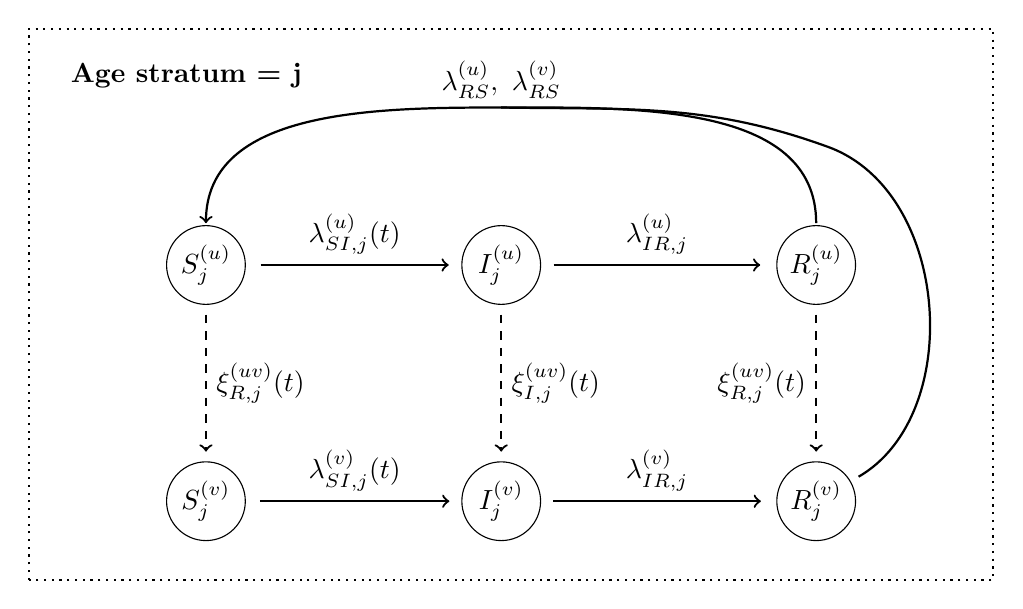
\begin{tikzpicture}
	\draw[thick,dotted] (-1,1) rectangle (11.25,8);
	\node at (1,7) [label={\textbf{Age stratum = j}}] {};
	\draw (1.25,5) circle(0.5) node (Sju) {$S_j^{(u)}$};
	\draw (5,5) circle(0.5) node (Iju) {$I_j^{(u)}$};
	\draw (9,5) circle(0.5) node (Rju) {$R_j^{(u)}$};
	\draw (1.25,2) circle(0.5) node (Sjv) {$S_j^{(v)}$};
	\draw (5,2) circle(0.5) node (Ijv) {$I_j^{(v)}$};
	\draw (9,2) circle(0.5) node (Rjv) {$R_j^{(v)}$};
	\draw (5,7) coordinate (rec) {};
	\draw (5,7.35) node (reclab) {$ \lambda_{RS}^{(u)},\ \lambda_{RS}^{(v)} $};
	\draw (9.15,6.5) coordinate (rec2) {};
	
	\draw [thick,shorten >=0.25cm,shorten <=0.25cm,->] (Sju) -- (Iju) node[midway,above] {$ \lambda_{SI,j}^{(u)}(t) $};
	\draw [thick,shorten >=0.25cm,shorten <=0.25cm,->] (Iju) -- (Rju) node[midway,above] {$ \lambda_{IR,j}^{(u)} $};
	\draw [thick,shorten >=0.25cm,shorten <=0.25cm,->] (Sjv) -- (Ijv) node[midway,above] {$ \lambda_{SI,j}^{(v)}(t) $};
	\draw [thick,shorten >=0.25cm,shorten <=0.25cm,->] (Ijv) -- (Rjv) node[midway,above] {$ \lambda_{IR,j}^{(v)} $};
	
	\draw [dashed,thick,shorten >=0.25cm,shorten <=0.25cm,->] (Sju) -- (Sjv) node[midway,right] {$ \xi_{R,j}^{(uv)}(t) $};
	\draw [dashed,thick,shorten >=0.25cm,shorten <=0.25cm,->] (Iju) -- (Ijv) node[midway,right] {$ \xi_{I,j}^{(uv)}(t) $};
	\draw [dashed,thick,shorten >=0.25cm,shorten <=0.25cm,->] (Rju) -- (Rjv) node[midway,left] {$ \xi_{R,j}^{(uv)}(t) $};
	
	\draw [thick,shorten >=0cm,shorten <=0.15cm] (Rju) to [out=90, in = 0] (rec);
	\draw [thick,shorten >=0cm,shorten <=0.1cm] (Rjv) to [out=30, in = -20] (rec2);
	\draw [thick] (rec2) to [out=160,in=-1] (rec);
	\draw [thick,shorten >=0.15cm,shorten <=0.0cm,->] (rec) to [out=180, in = 90] (Sju);
		
	\end{tikzpicture}
\end{center}

\subsection{Flexible Models for the Force of Infection with Gaussian Markov Random Fields}
\label{subsec:flu_gmrf}


\section{Discussion}